\documentclass{standalone}
\usepackage{tikz}
\usetikzlibrary{arrows.meta, positioning, shapes.geometric}

\begin{document}
	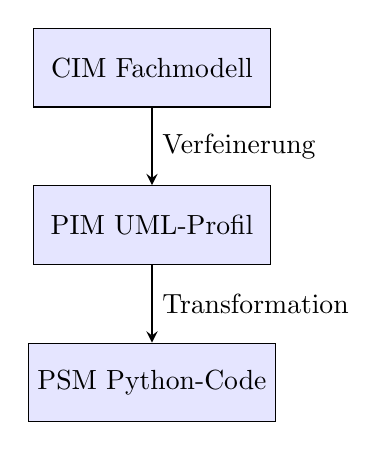
\begin{tikzpicture}[
		node distance=2cm,
		box/.style={rectangle, draw, fill=blue!10, minimum width=3cm, minimum height=1cm, text centered},
		arrow/.style={->, >=stealth, thick}
		]
		\node[box] (cim) {CIM Fachmodell};
		\node[box, below of=cim] (pim) {PIM UML-Profil};
		\node[box, below of=pim] (psm) {PSM Python-Code};
		
		\draw[arrow] (cim) -- (pim) node[midway, right] {Verfeinerung};
		\draw[arrow] (pim) -- (psm) node[midway, right] {Transformation};
	\end{tikzpicture}
\end{document}